Le circuit que nous allons utiliser aujourd'hui se compose de quatre éléments:
\begin{enumerate}
  \item D'une télécommande infrarouges
  \item Récepteur infrarouges
  \item Une led
  \item L'Arduino qui est le \textit{"cerveau"} du système. Il allume la Led quand la télécommande lui demande.
\end{enumerate}

Pour que tout ceci fonctionne, la première étape est d'assembler tout ces composants sur une breadboard. Le schéma du circuit est disponible à la \ref{fig:circuit}.

\begin{figure}[!t]
\centering
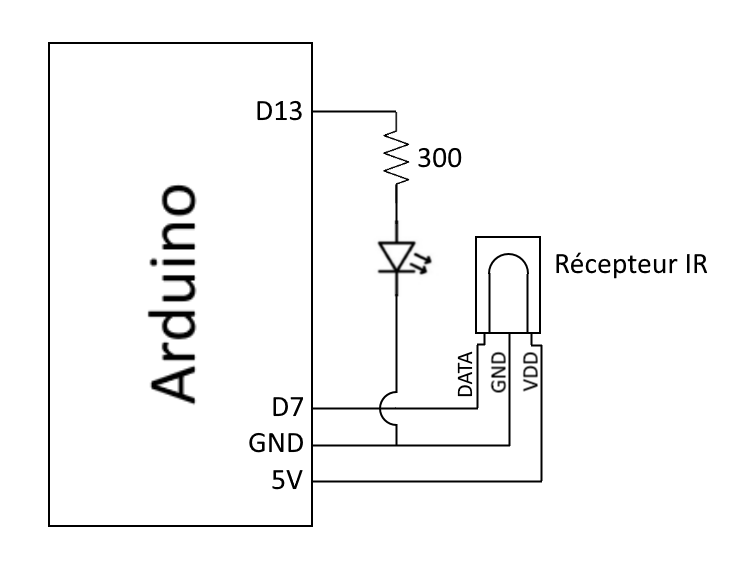
\includegraphics[width=0.8\textwidth]{imgs/circuit.png}
\caption{Circuit à réaliser pour contrôler l'Arduino grâce à une télécommande infrarouge.}
\label{fig:circuit}
\end{figure}
